\begin{frame}{How to find genuine decays? \textemdash Example \decay{\Lz}{\proton\pim}}
    \begin{columns}
        \begin{column}{.55\textwidth}
            \begin{itemize}
                \item Create \Lz candidates: $\{\Lz\} := \{\proton\} \otimes \{\pim\}$
                \item Use inv.\ mass $m(\Lz)\ftnt{} \overset{?}{=} m(\proton\pim)$ as proxy
                \item Separate components:
                \begin{enumerate}
                    \item Combinatorial background \\ \scalebox{.8}{(random track combinations)}
                    \item physical background \\ \scalebox{.8}{(\eg{}, \decay{\KS}{\textcolor{vertexDarkRed}{\pip}\pim})}
                    \item genuine \decay{\Lz}{\proton\pim} decays
                \end{enumerate}
            \end{itemize}
        \end{column}
        \begin{column}{.45\textwidth}
            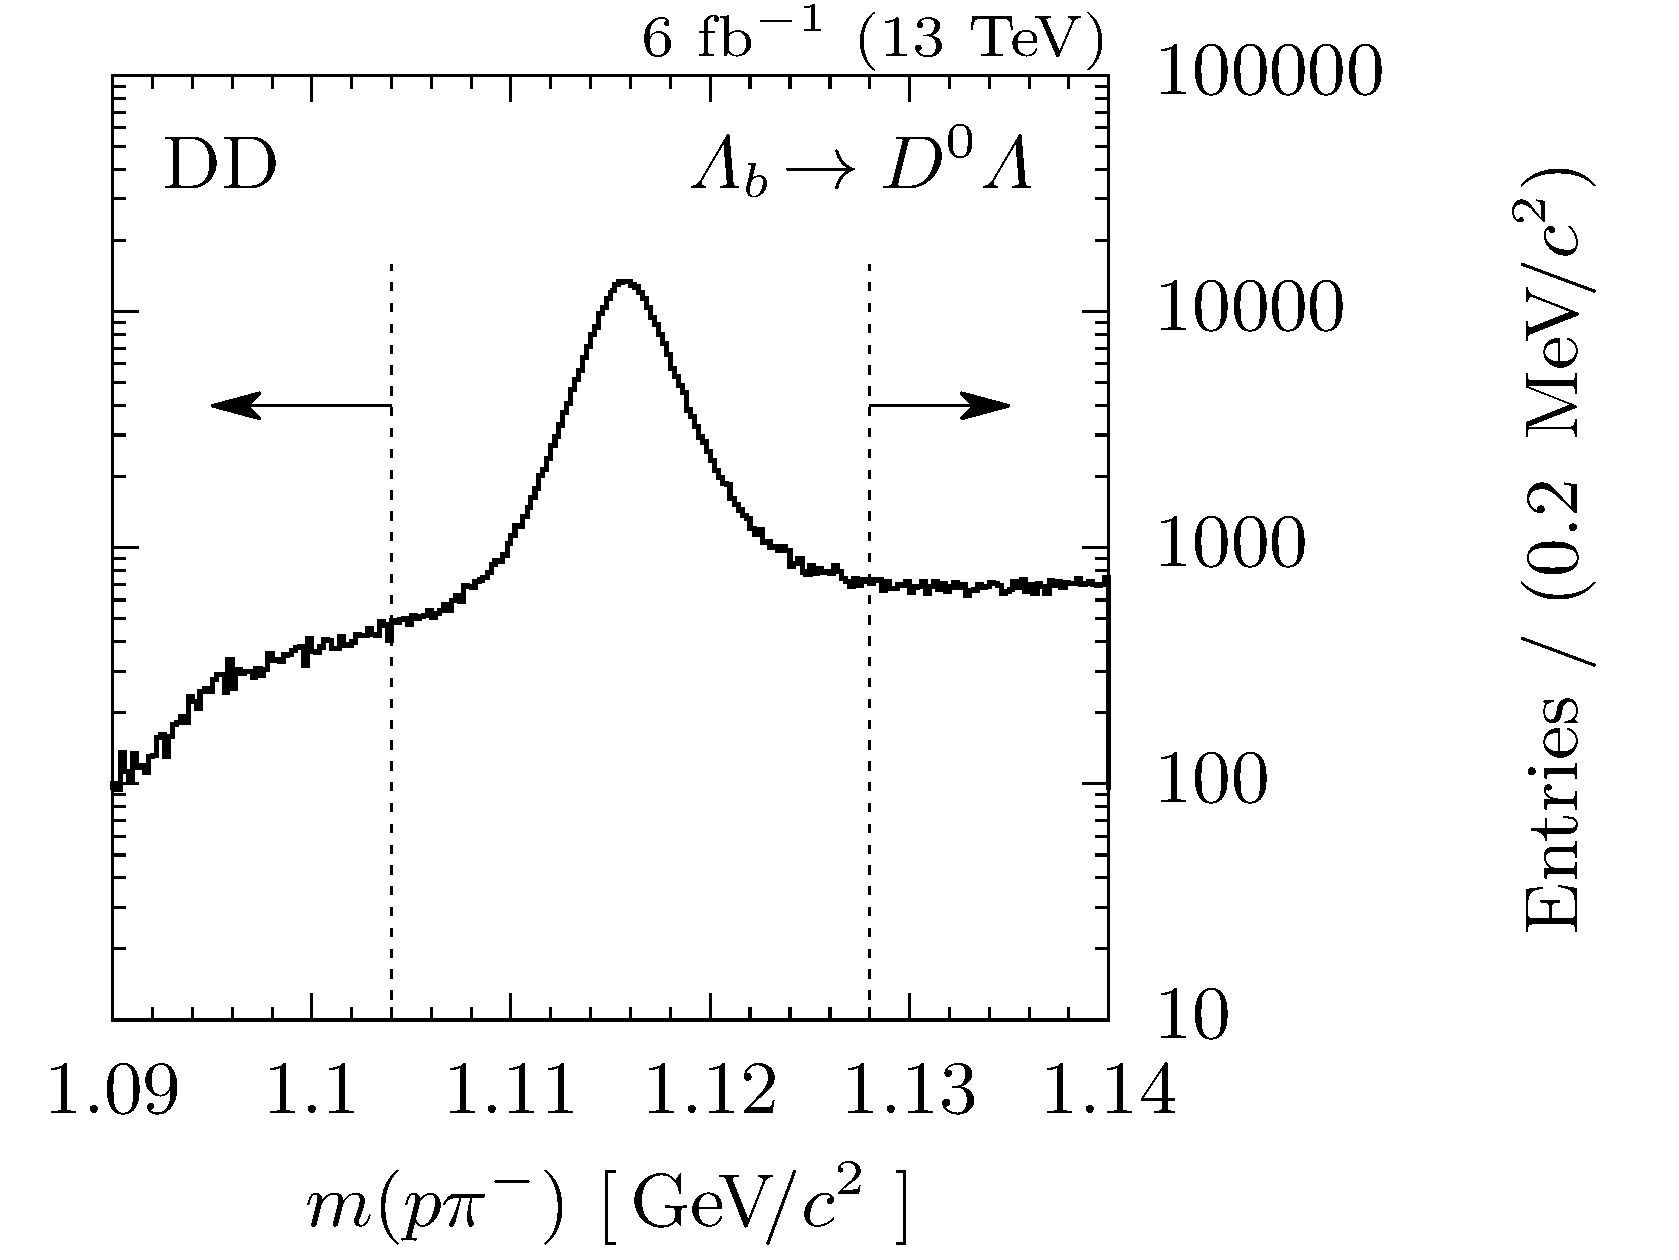
\includegraphics[width=\textwidth]{mvaLz/hLzM_DD}\\
            \hspace{5mm} \footnotesize (\ftnt PDG: $m(\Lz) \approx 1.117\gevcc$)
        \end{column}
    \end{columns}

    \vspace{5mm}

    \scalebox{0.8}{\vbox{%
    Technical detail: only (weak) Cabibbo suppressed decays possible for \Lz
    \vspace{-2mm}
    \begin{itemize}
        \item \textit{long} lifetime
        \item some \Lz decay outside (inside) of first detector element: refer to as \textbf{DD} (\textbf{LL})
        \item different detector response, separate analysis necessary
    \end{itemize}}}
\end{frame}

\begin{frame}[plain,noframenumbering]
    \centering
    \scalebox{2.}{Do the same for \decay{\Lb/\Xibz}{\Dz\Lz}?}

    \ie{}, $\{ \Lb/\Xibz \} := \underbrace{\{ \Km \} \otimes \{ \pip \}}_{\{ \Dz \}} \otimes \underbrace{\{ \proton \} \otimes \{ \pim \}}_{\{ \Lz \}}$
\end{frame}

\begin{frame}{Searching for \decay{\Lb/\Xibz}{\Dz\Lz}}
    \begin{columns}
        \begin{column}{.55\textwidth}
            \textbf{No signal visible!}
            \begin{itemize}
                \item Background (at this stage) mainly combinatorial
                \item Need to increase
                \begin{itemize}
                    \item purity of $\{ \Dz \}$
                    \item purity of $\{ \Lz \}$
                    \item filter $\{ \Dz \} \otimes \{ \Lz \}$ for $\decay{\Lb/\Xibz}{\Dz\Lz}$ decays by constraining physical properties
                \end{itemize}
                \item (Carefully analyse physical backgrounds\ftntdagger)
            \end{itemize}
        \end{column}
        \begin{column}{.45\textwidth}
            \only<1>{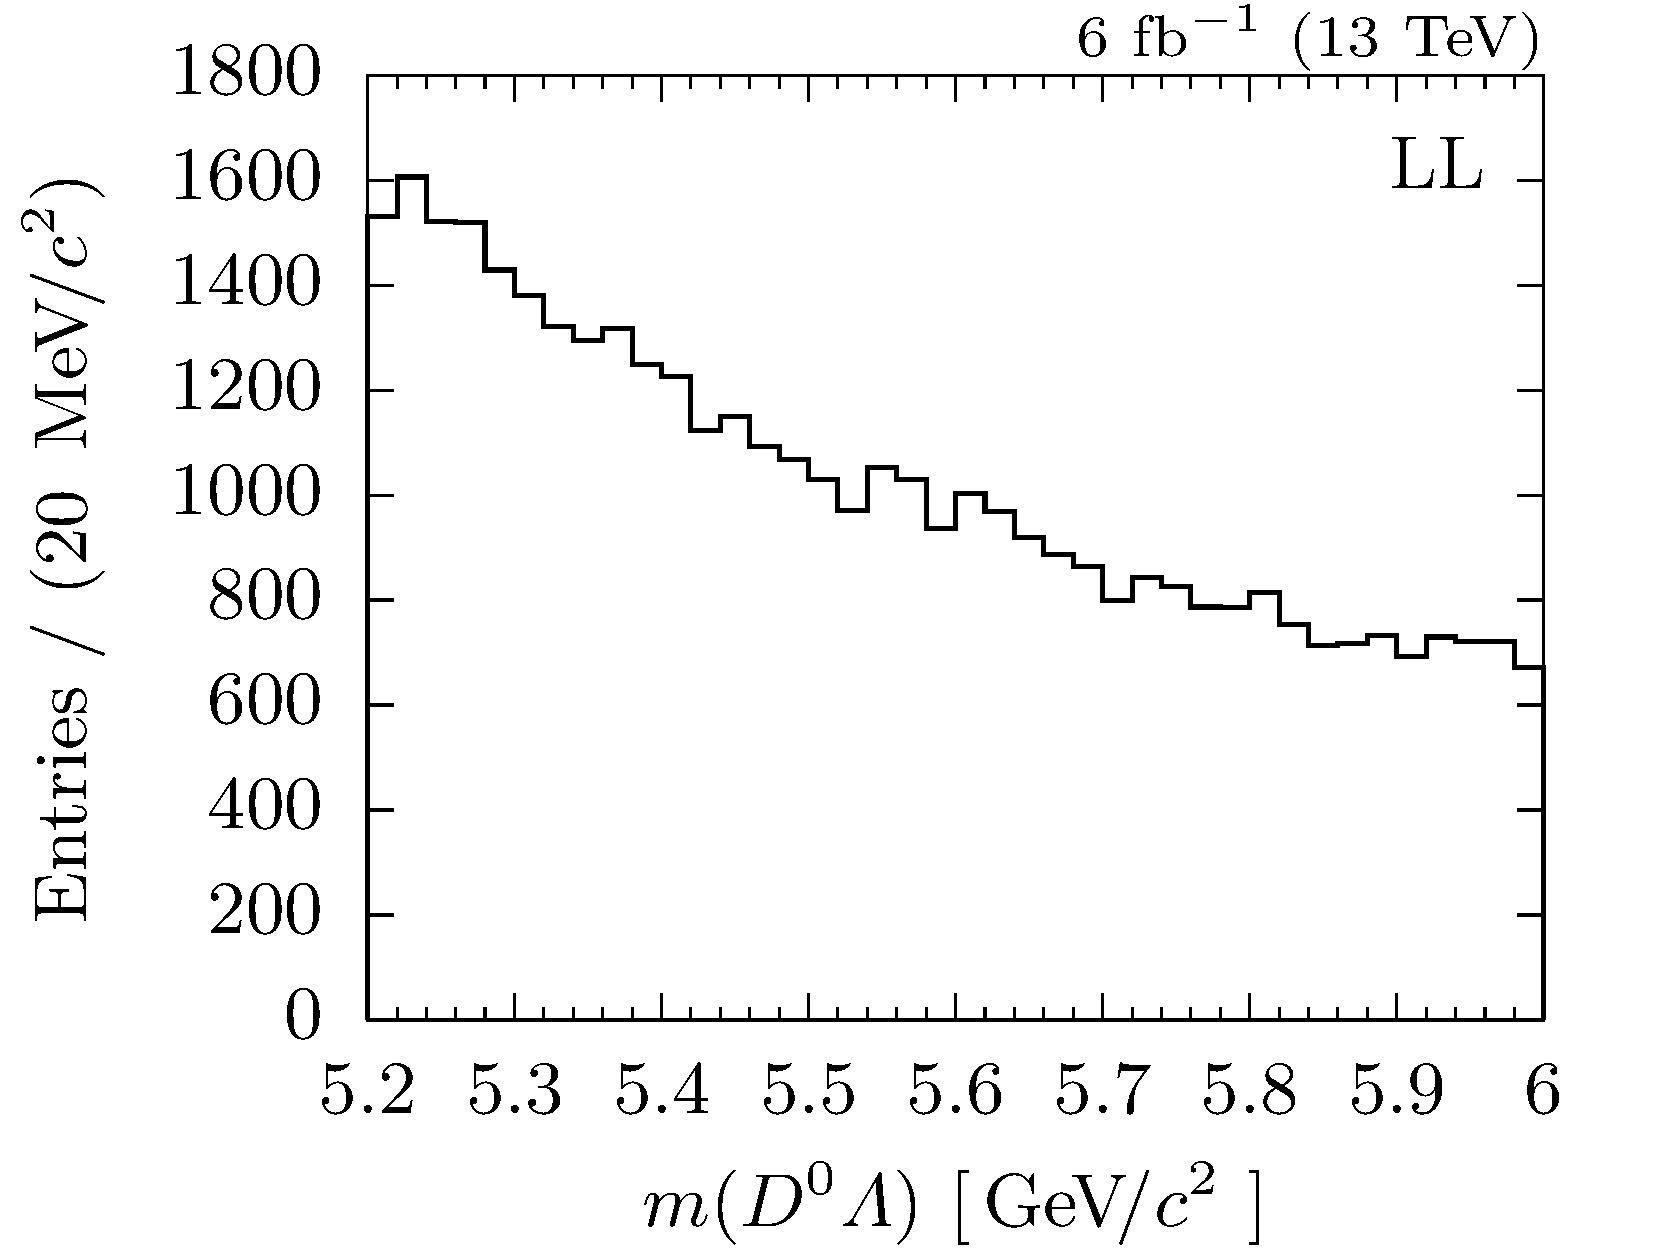
\includegraphics[width=\textwidth]{mvaLbDz/hDzLzM_LL}}%
            \only<2>{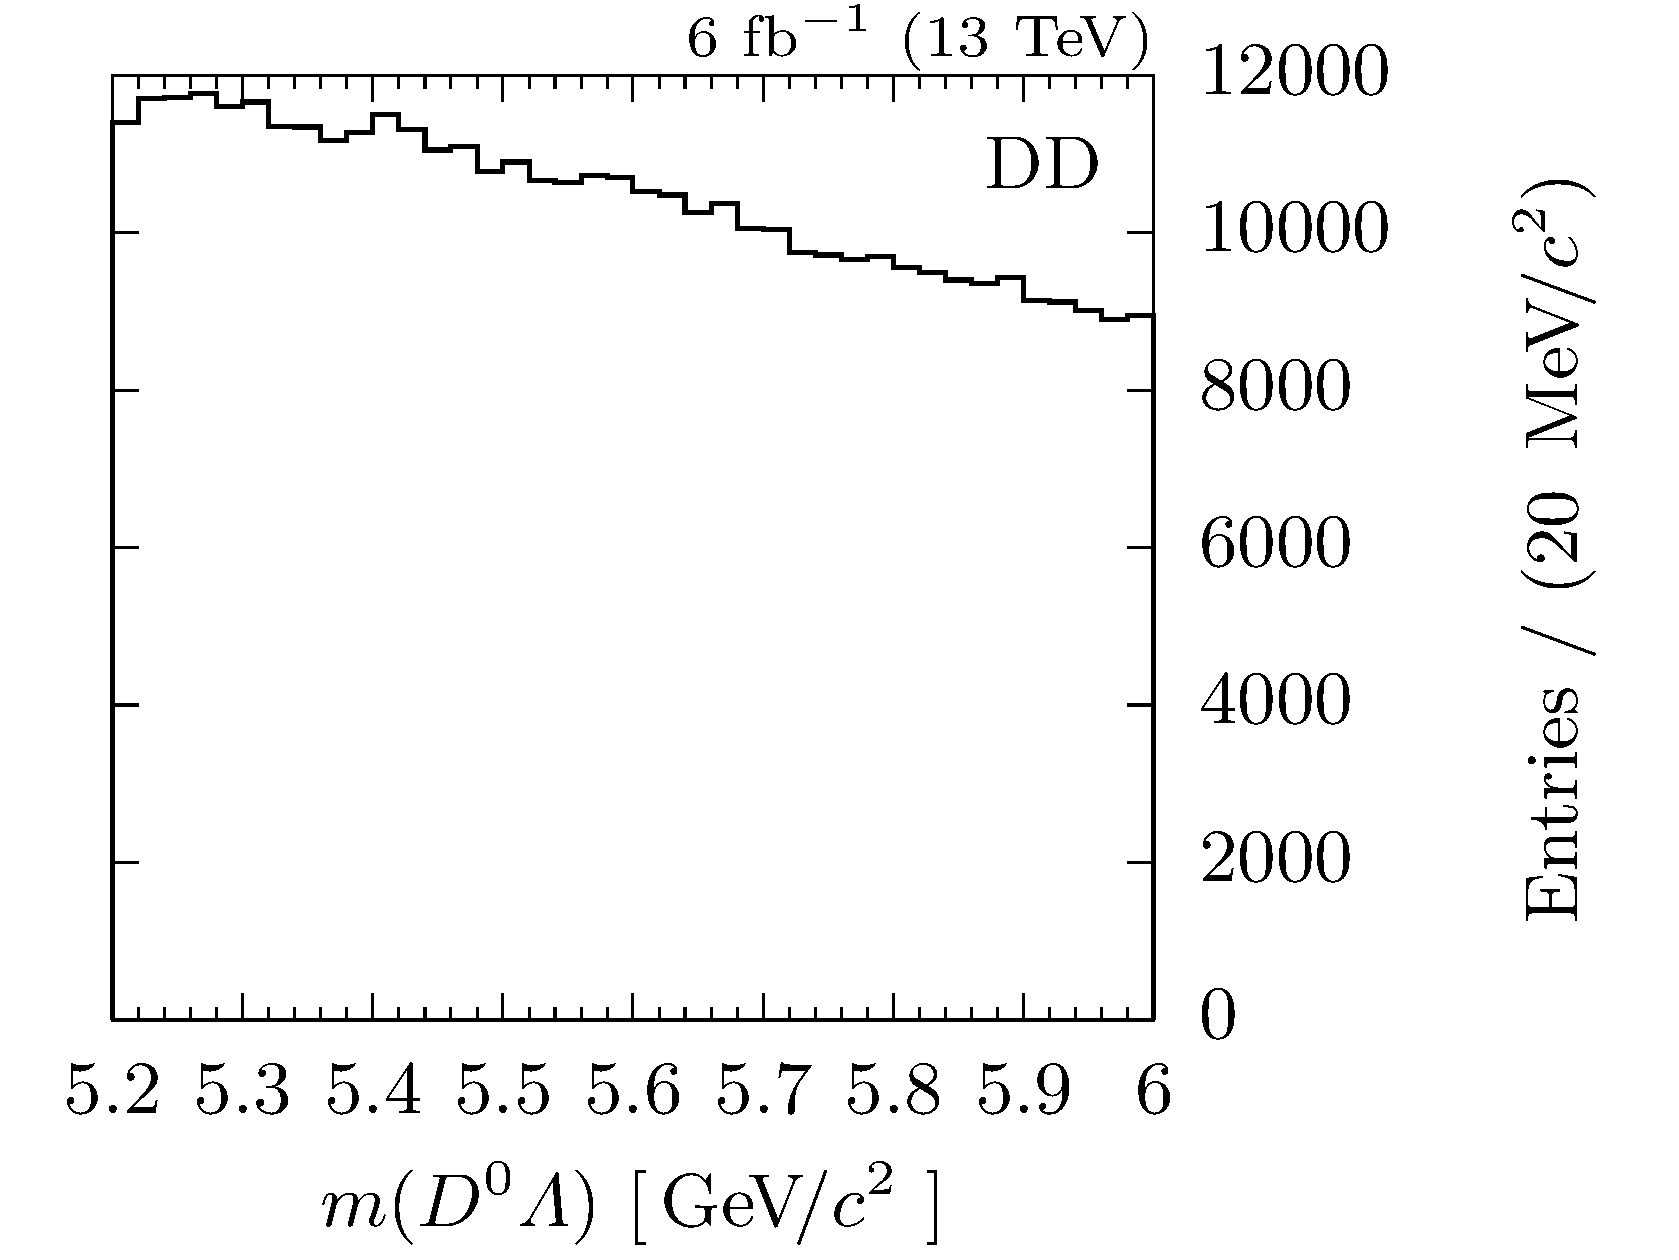
\includegraphics[width=\textwidth]{mvaLbDz/hDzLzM_DD}}%
            \\
            \hspace{5mm} \footnotesize (PDG: $m(\Lb) \approx 5.620\gevcc$,\\
            \hspace{5mm} \footnotesize \phantom{(}PDG: $m(\Xibz) \approx 5.792\gevcc$)
        \end{column}
    \end{columns}
\end{frame}

\begin{frame}{Searching for \decay{\Lb/\Xibz}{\Dz\Lz}}
    \begin{columns}
        \begin{column}{.6\textwidth}
            \textbf{Use ML to rescue!} Classification problem
            \begin{itemize}
                \item Separate \textit{\textbf{signal}} (genuine \decay{\Lb/\Xibz}{\Dz\Lz})
                \item \ldots from (combinatorial) \textit{\textbf{background}}
                \item Labels?
                \begin{itemize}
                    \item use MC simulated decays for class \textit{signal}\ftntdagger{}
                    \item use recorded data from sidebands for class \textit{background}
                \end{itemize}
            \end{itemize}
        \end{column}
        \begin{column}{.4\textwidth}
            \centering
            
\includegraphics[width=.5\textwidth]{needle_haystack}\\
            {\tiny (Image: R.~Diepenheim on \texttt{thenounproject.com})}
        \end{column}
    \end{columns}

    \vspace{5mm}

    \footnotesize \ftntdagger{} calibration needed (not discussed here)
\end{frame}

\begin{frame}{MVA methodoloy}
    \begin{tikzpicture}[>=triangle 45,
                        node/.style={rectangle,align=center,rounded corners}]
        \node[draw,node] (data) {$X, y, w$};
        \node[draw,node,right=1cm of data] (presel) {Loose / \\ (pre-)selection\ftntdagger};
        \node[draw,node,right=2cm of presel] (pProbNNp) {\texttt{ProbNNp}\ftnt{}};
        \node[draw,node,above=.5cm of pProbNNp] (clfLbDz) {\Lb-\Dz classifier};
        \node[draw,node,above=.5cm of clfLbDz] (clfLz) {\Lz classifier};
        \node[draw,node,below=.5cm of pProbNNp] (kProbNNk) {\texttt{ProbNNk}\ftnt{}};
        \node[draw,node,below=.5cm of kProbNNk] (dtf) {DTF prob.};
        \node[draw,node,right=2cm of pProbNNp] (fclf) {Rectangular\\ cut classifier};

        \draw[->] (data) -- (presel);
        \draw[->] (presel) -- (pProbNNp);
        \draw[->] (presel.north east) + (0,-1mm) -- (clfLz.west);
        \draw[->] (presel.north east) + (0,-3mm) -- (clfLbDz.west);
        \draw[->] (presel.south east) + (0, 3mm) -- (kProbNNk.west);
        \draw[->] (presel.south east) + (0, 1mm) -- (dtf.west);
        \draw[->] (pProbNNp) -- (fclf);
        \draw[->] (clfLz.east) -- ($(fclf.north west) + (0,-1mm)$);
        \draw[->] (clfLbDz.east) -- ($(fclf.north west) + (0,-3mm)$);
        \draw[->] (kProbNNk.east) -- ($(fclf.south west) + (0,3mm)$);
        \draw[->] (dtf.east) -- ($(fclf.south west) + (0,1mm)$);
    \end{tikzpicture}

    \textbf{Training:} classify $m$ data $X \in \mathbb{R}^{m \times n}$ with $n$ features using labels $y \in \{ \text{sig.}, \text{bkg.} \}^m$ and calibration factors\ftntdagger{} $w \in \mathbb{R}^m$ with $\mathcal{O}(m) = 10k$, $n = 18$

    \vspace{5mm}
    \footnotesize \ftnt{} pre-trained shallow NN
\end{frame}

\begin{frame}{Example: \Lz classifier}
    \begin{columns}
        \begin{column}{.55\textwidth}
            \begin{itemize}
                \item 5 features of $\{ \Lz \}$: 
                \begin{enumerate}
                    \item transverse momentum
                    \item angle between momentum and connecting line between \proton\proton-IA point (PV) and \Lz decay vertex
                    \item $\chi^2$ improvement of PV with \Lz track
                    \item fit prob.\ of decay vertex
                    \item significance of flight distance
                \end{enumerate}
                \item Separate classifiers for LL and DD
                \item Optimize hyper-parameters of 5 classifiers using grid search w.r.t.\ ROC-AUC\ftnt{} value
            \end{itemize}
        \end{column}
        \begin{column}{.45\textwidth}
            \centering
            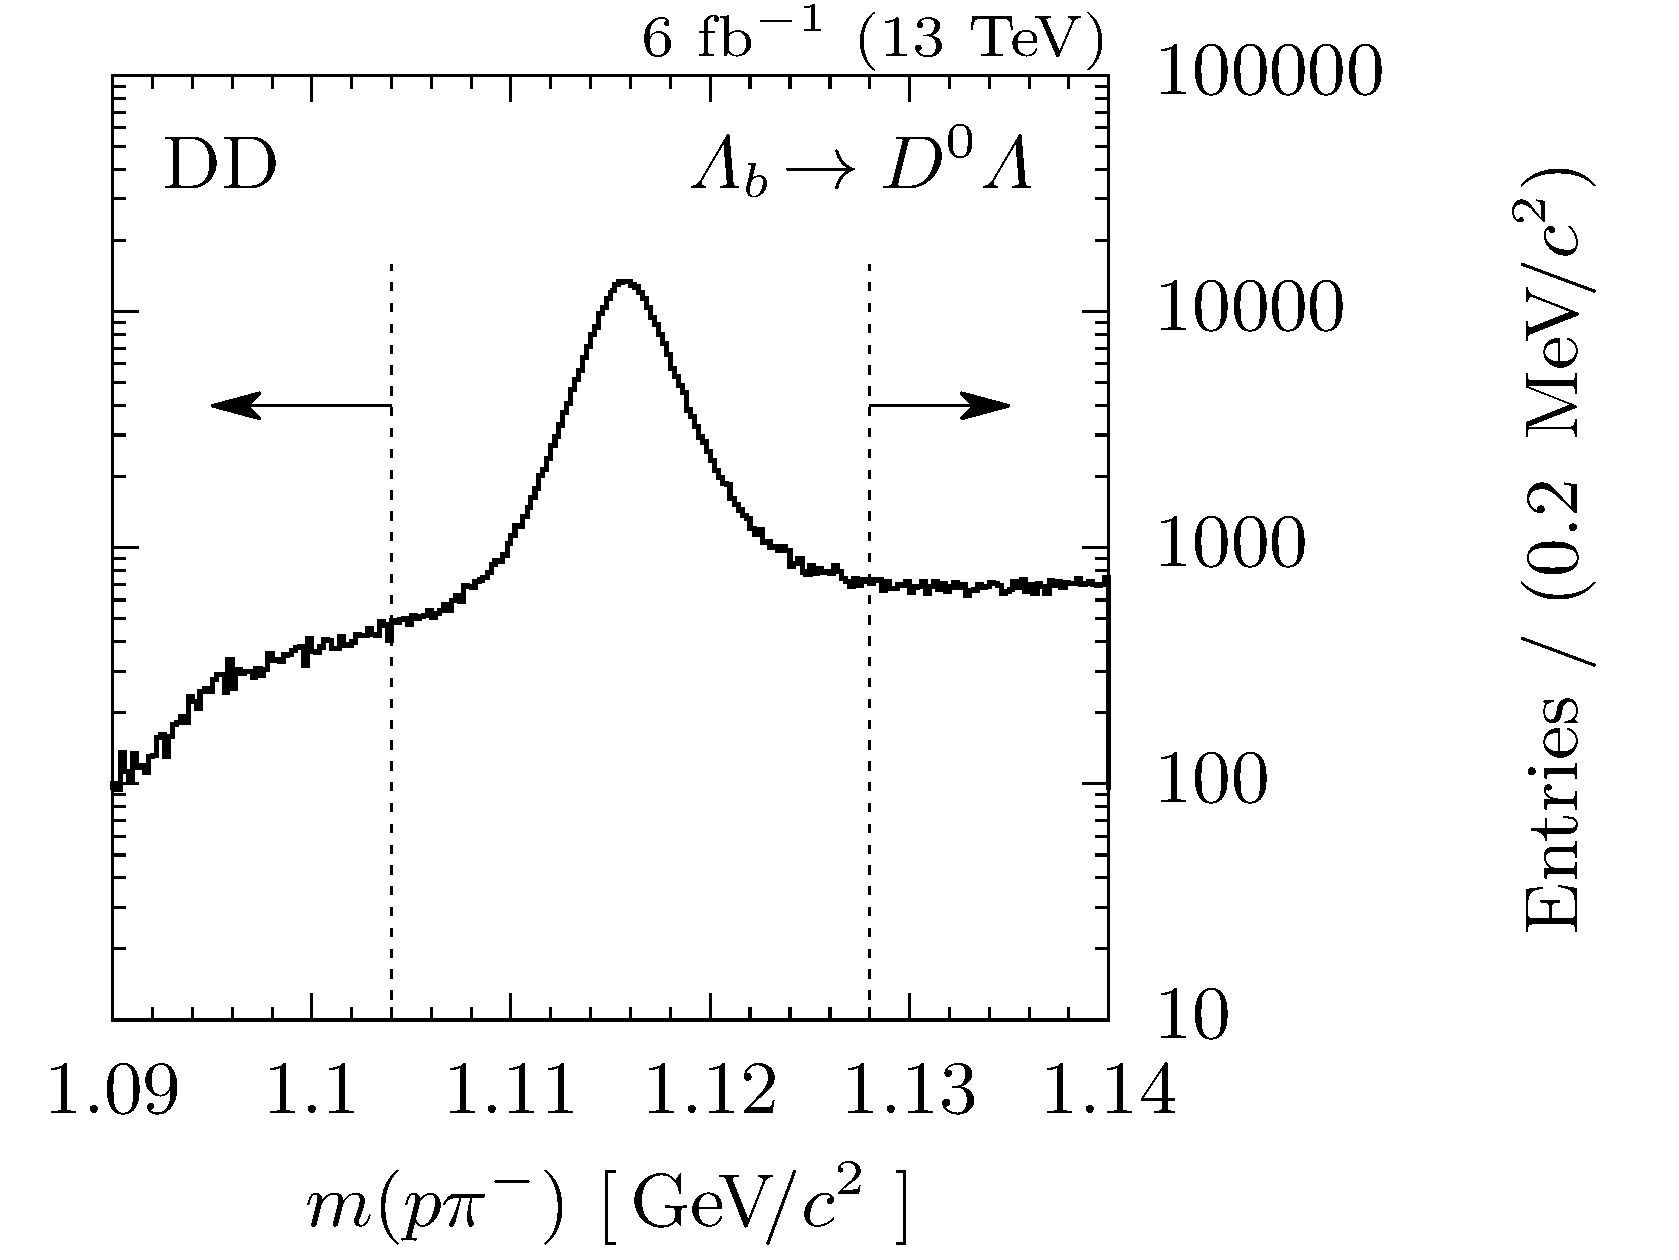
\includegraphics[scale=1.]{mvaLz/hLzM_DD}
        \end{column}
    \end{columns}

    \vspace{5mm}
    \footnotesize \ftnt{} Prob.\ that clf.\ will rank randomly chosen \textit{sig.} instance higher than randomly chosen \textit{bkg.} one
\end{frame}

\begin{frame}{Example: \Lz classifier}
    \begin{columns}
        \begin{column}{.45\textwidth}
            \scalebox{1.2}{\Lz classifier}
            \begin{itemize}
                \item \textcolor{vertexDarkRed}{5 features of $\{ \Lz \}$}
                \item Separate classifiers for LL and \textbf{DD}
                \item Optimize hyper-parameters of 5 classifiers using grid search w.r.t.\ ROC-AUC\ftnt{} value
            \end{itemize}
        \end{column}
        \begin{column}{.5\textwidth}
            \centering
            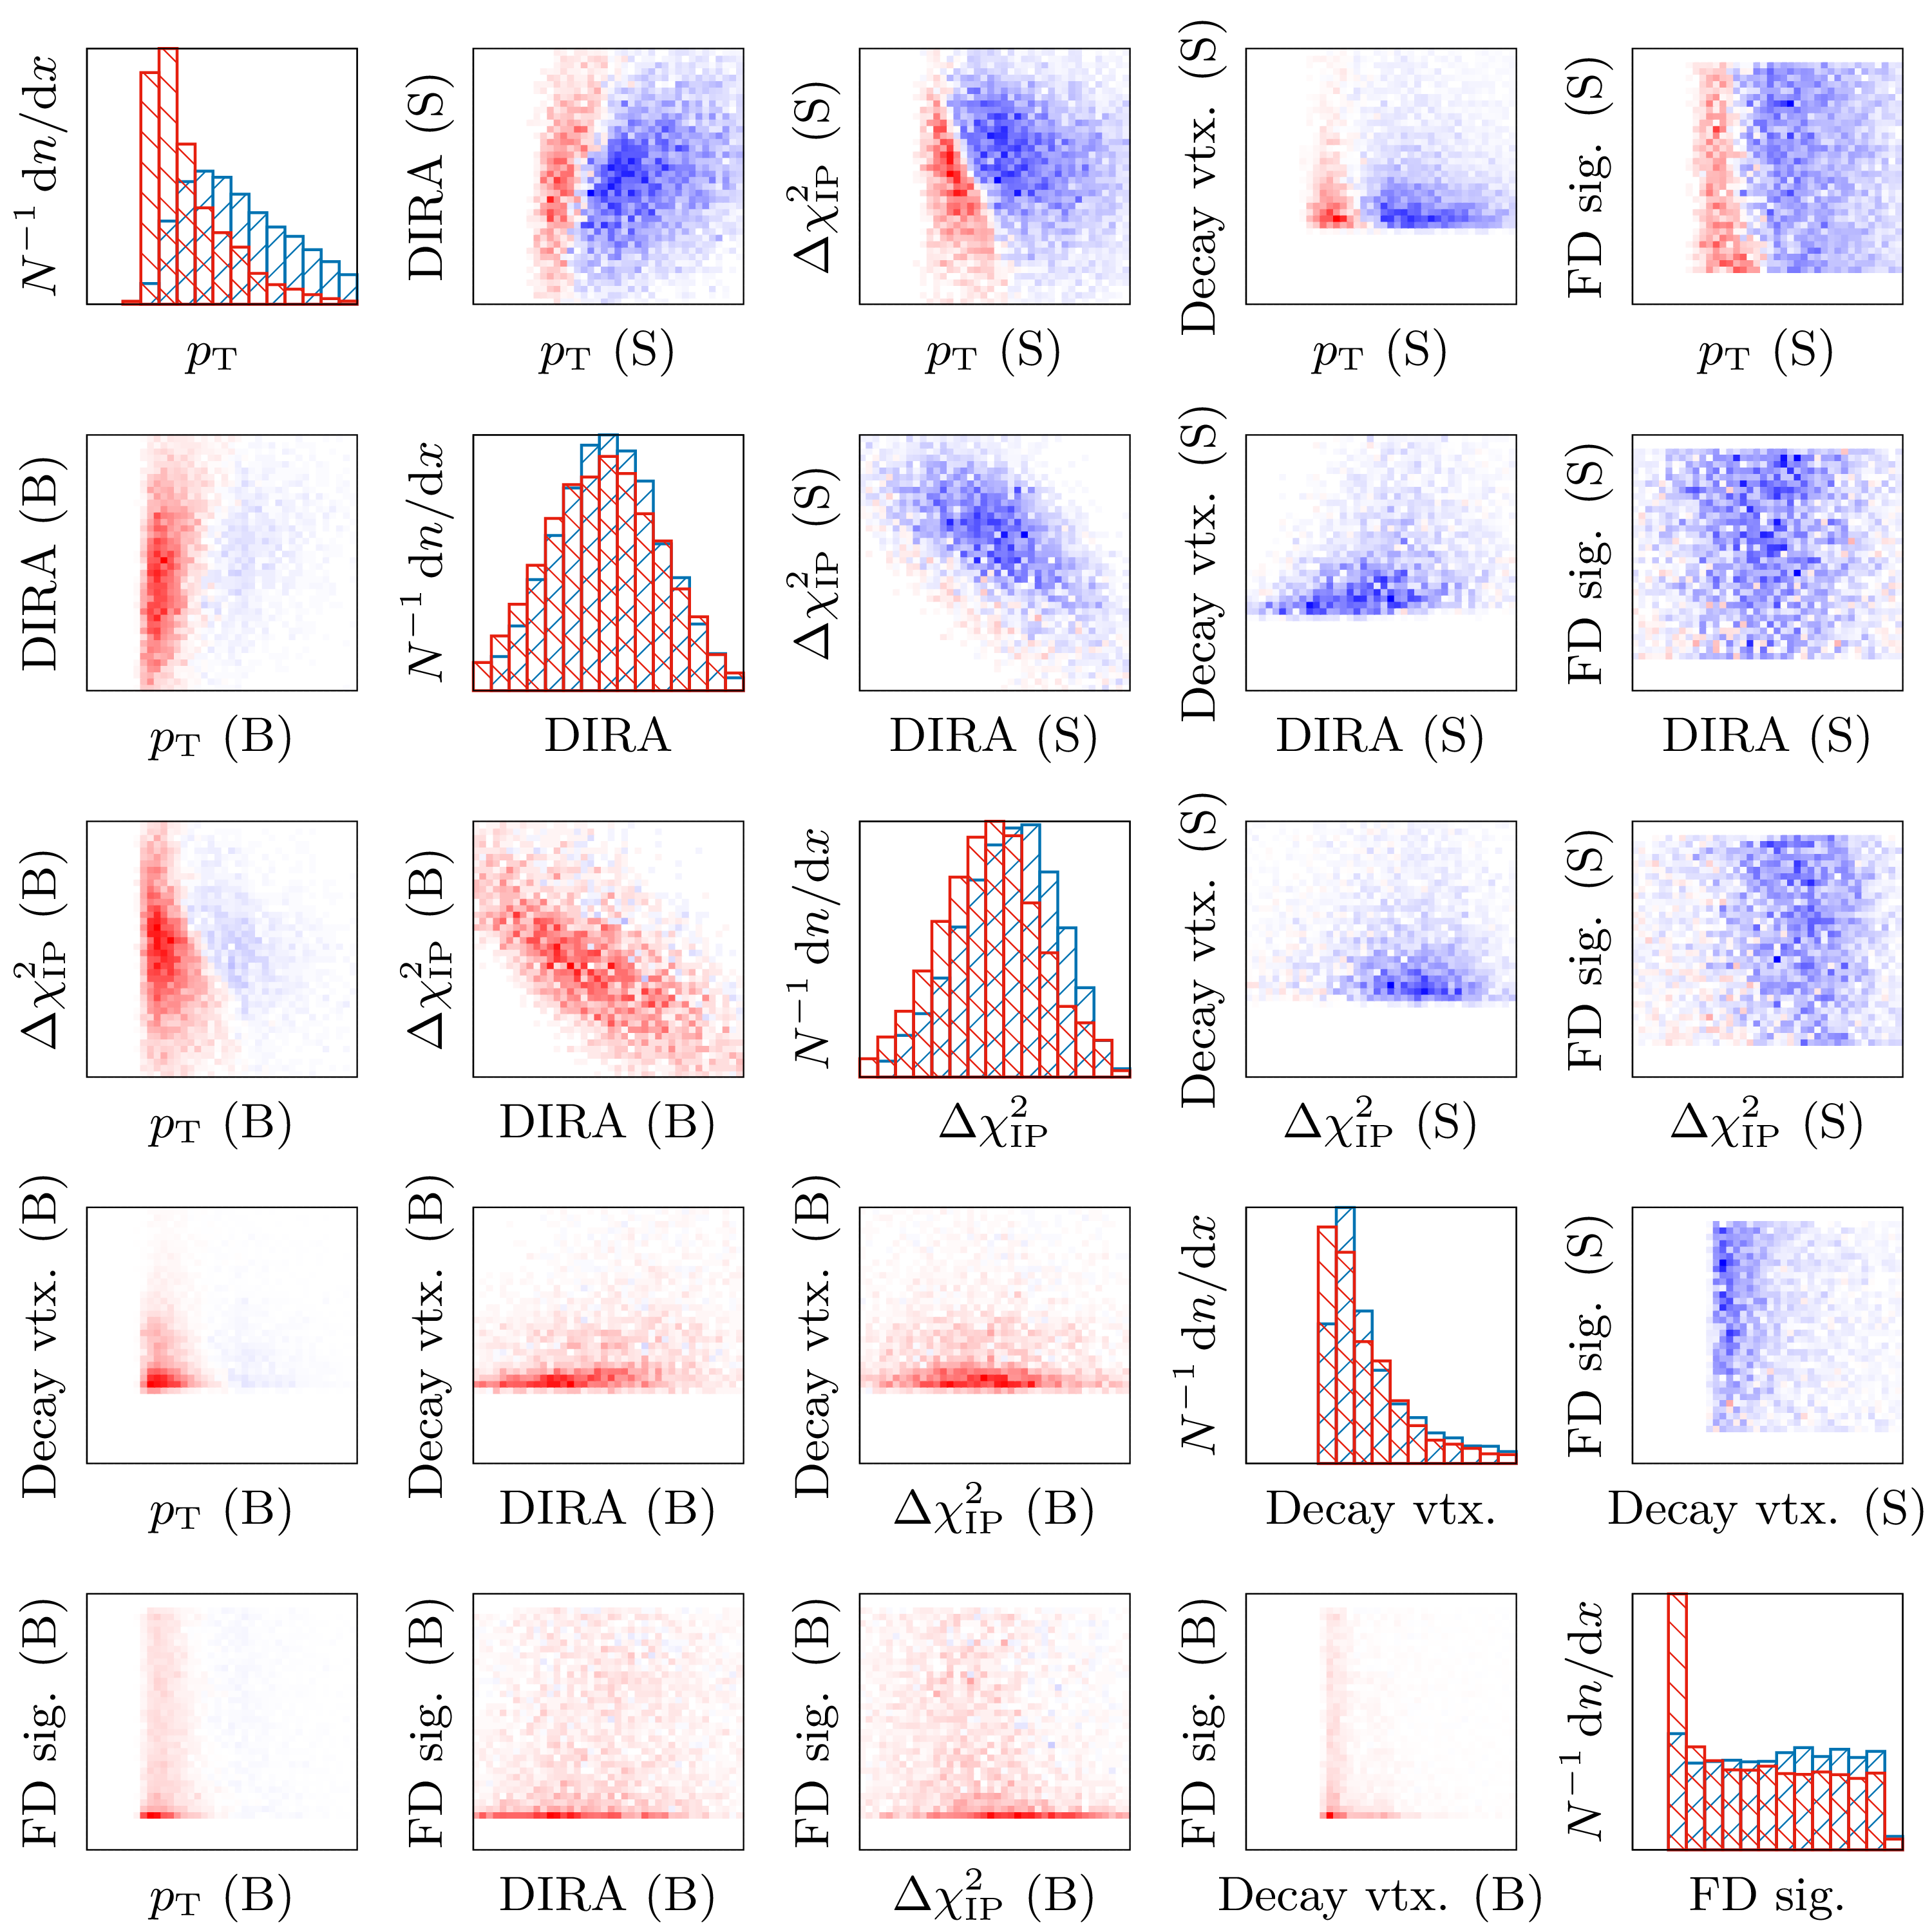
\includegraphics[height=.9\textheight]{mvaLz/mvaLz_corr_DD}\\
            (track type \textbf{DD})
        \end{column}
    \end{columns}
\end{frame}

\begin{frame}{Example: \Lz classifier}
    \begin{columns}
        \begin{column}{.45\textwidth}
            \scalebox{1.2}{\Lz classifier}
            \begin{itemize}
                \item 5 features of $\{ \Lz \}$
                \item Separate classifiers for LL and \textbf{DD}
                \item Optimize hyper-parameters of \textcolor{vertexDarkRed}{5 classifiers} using grid search w.r.t.\ ROC-AUC\ftnt{} value
            \end{itemize}
        \end{column}
        \begin{column}{.5\textwidth}
            \centering
            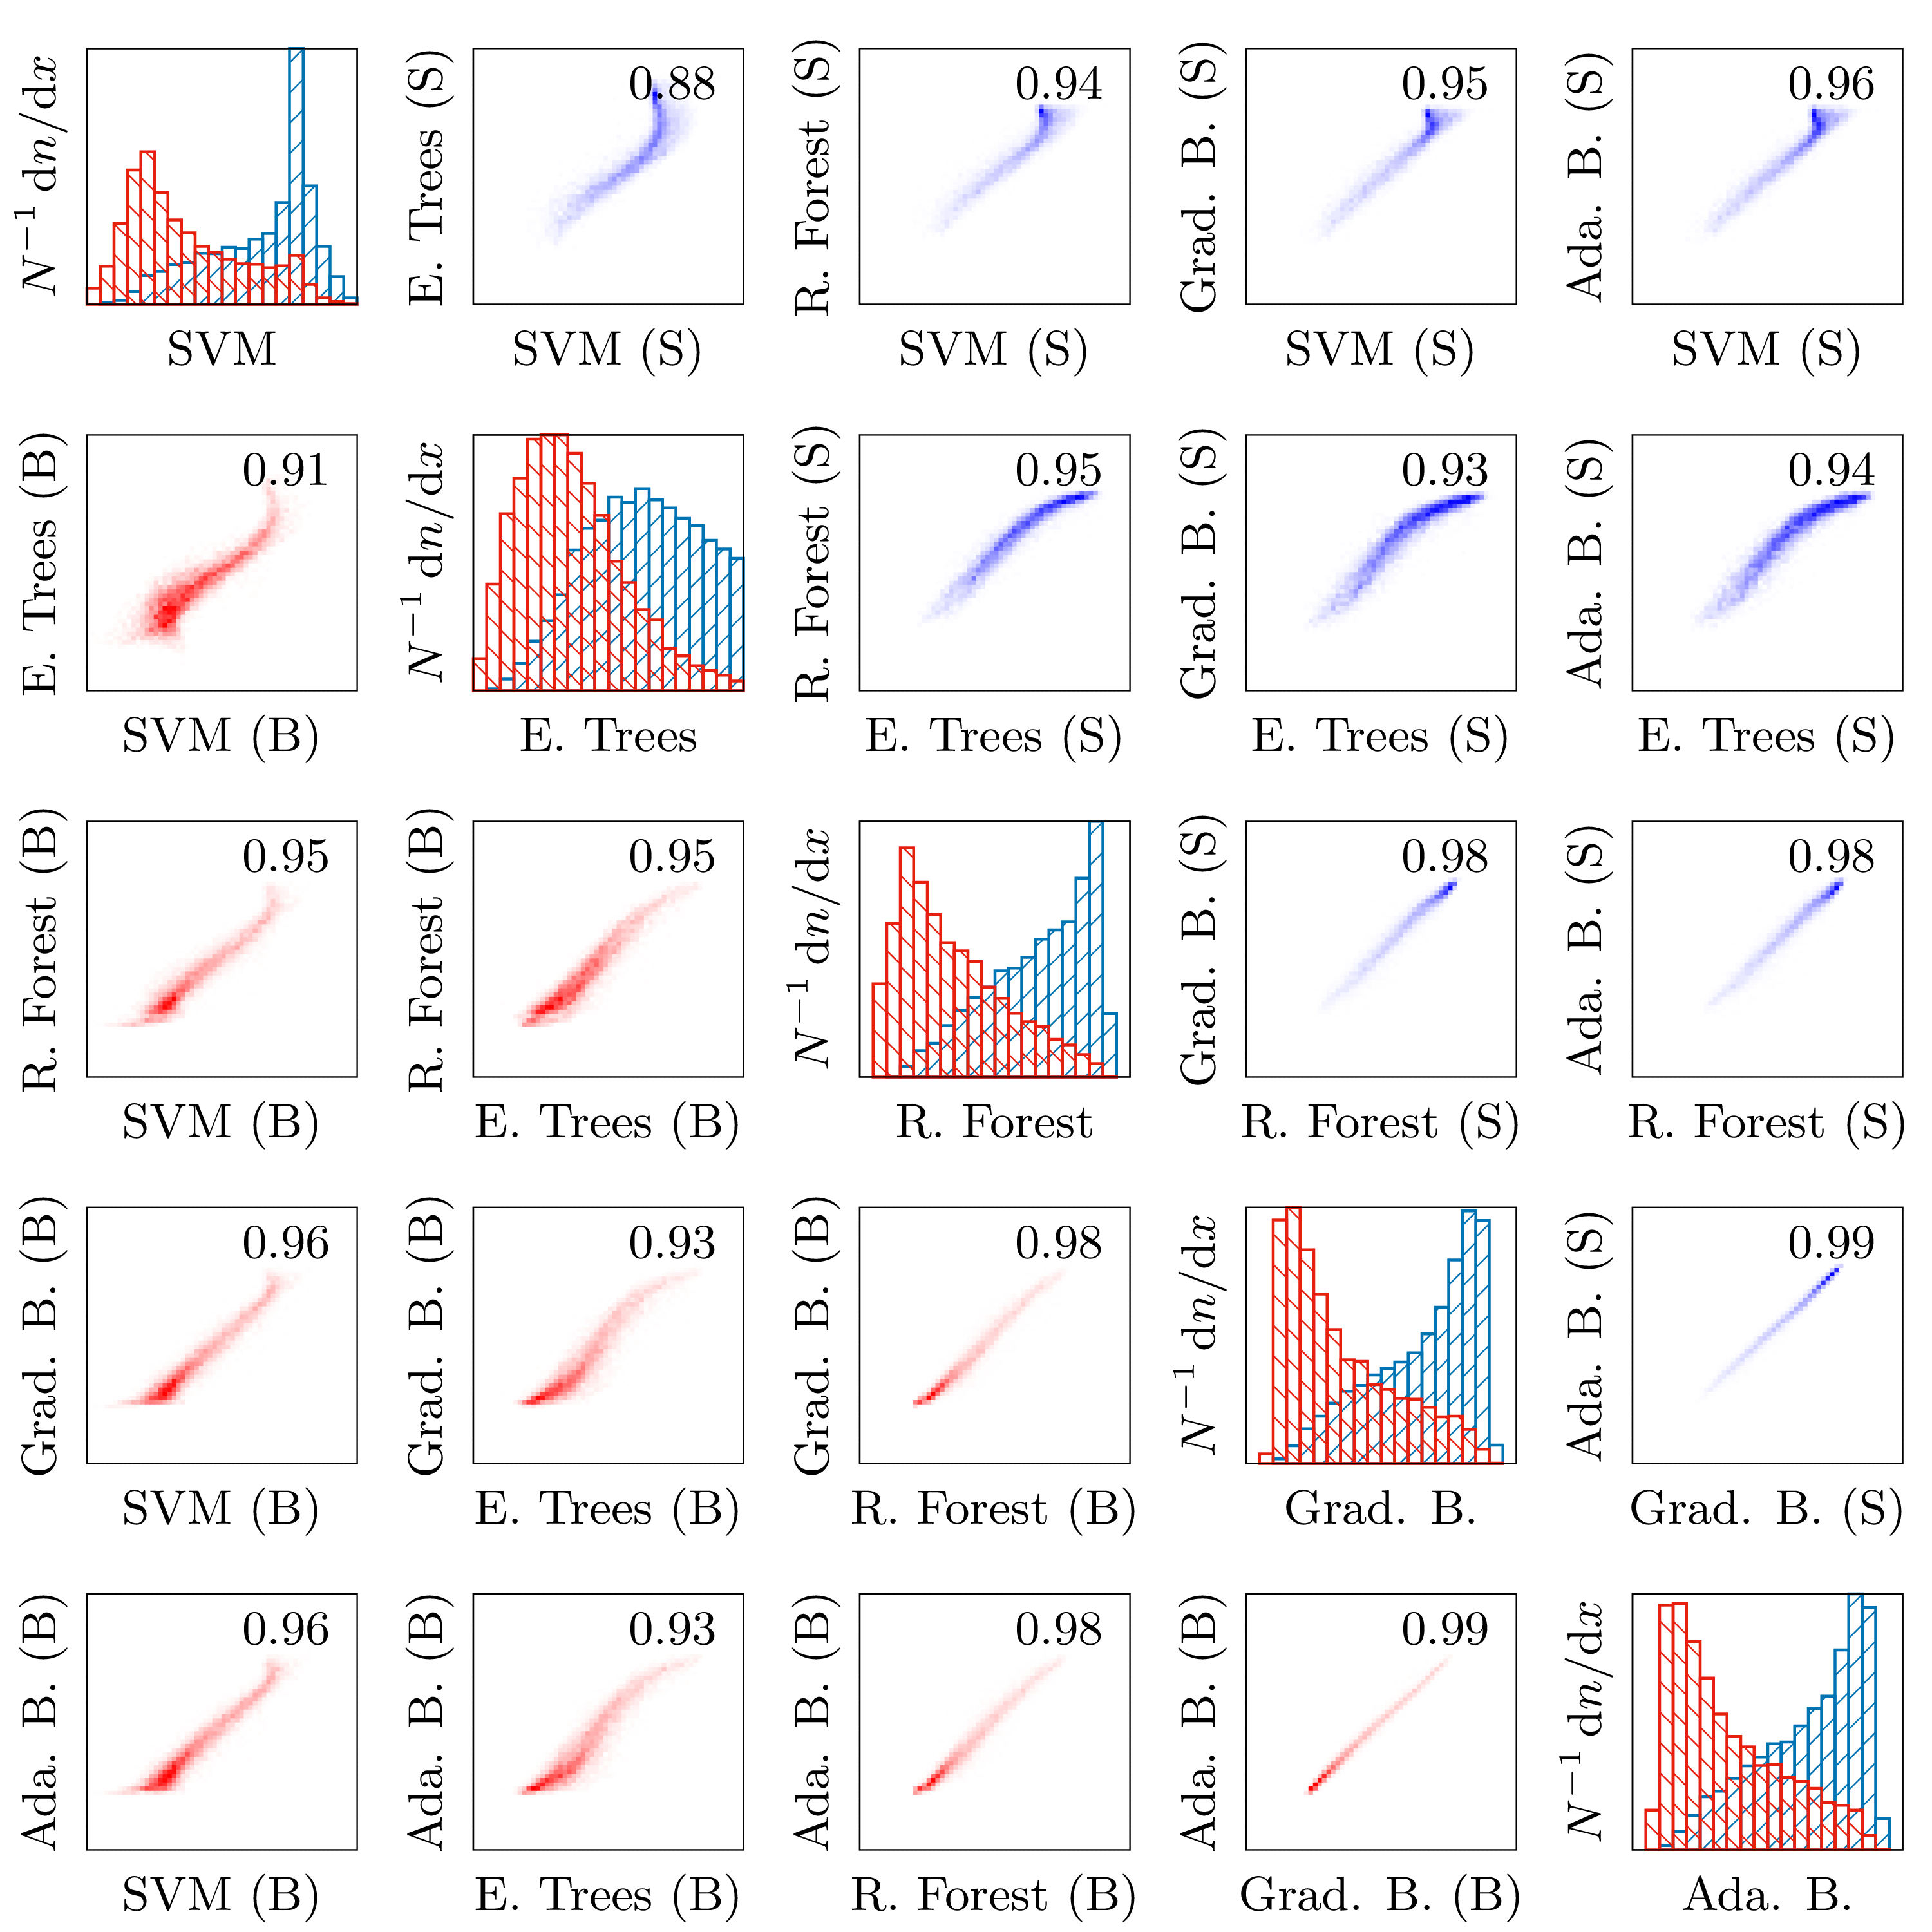
\includegraphics[height=.9\textheight]{mvaLz/stack_features_DD}\\
            (track type \textbf{DD})
        \end{column}
    \end{columns}
\end{frame}

\begin{frame}{Example: \Lz classifier}
    \begin{columns}
        \begin{column}{.45\textwidth}
            \scalebox{1.2}{\Lz classifier}
            \begin{itemize}
                \item 5 features of $\{ \Lz \}$
                \item Separate classifiers for LL and \textbf{DD}
                \item Optimize hyper-parameters of \textcolor{vertexDarkRed}{5 classifiers} using grid search w.r.t.\ ROC-AUC\ftnt{} value
            \end{itemize}
        \end{column}
        \begin{column}{.5\textwidth}
            \centering
            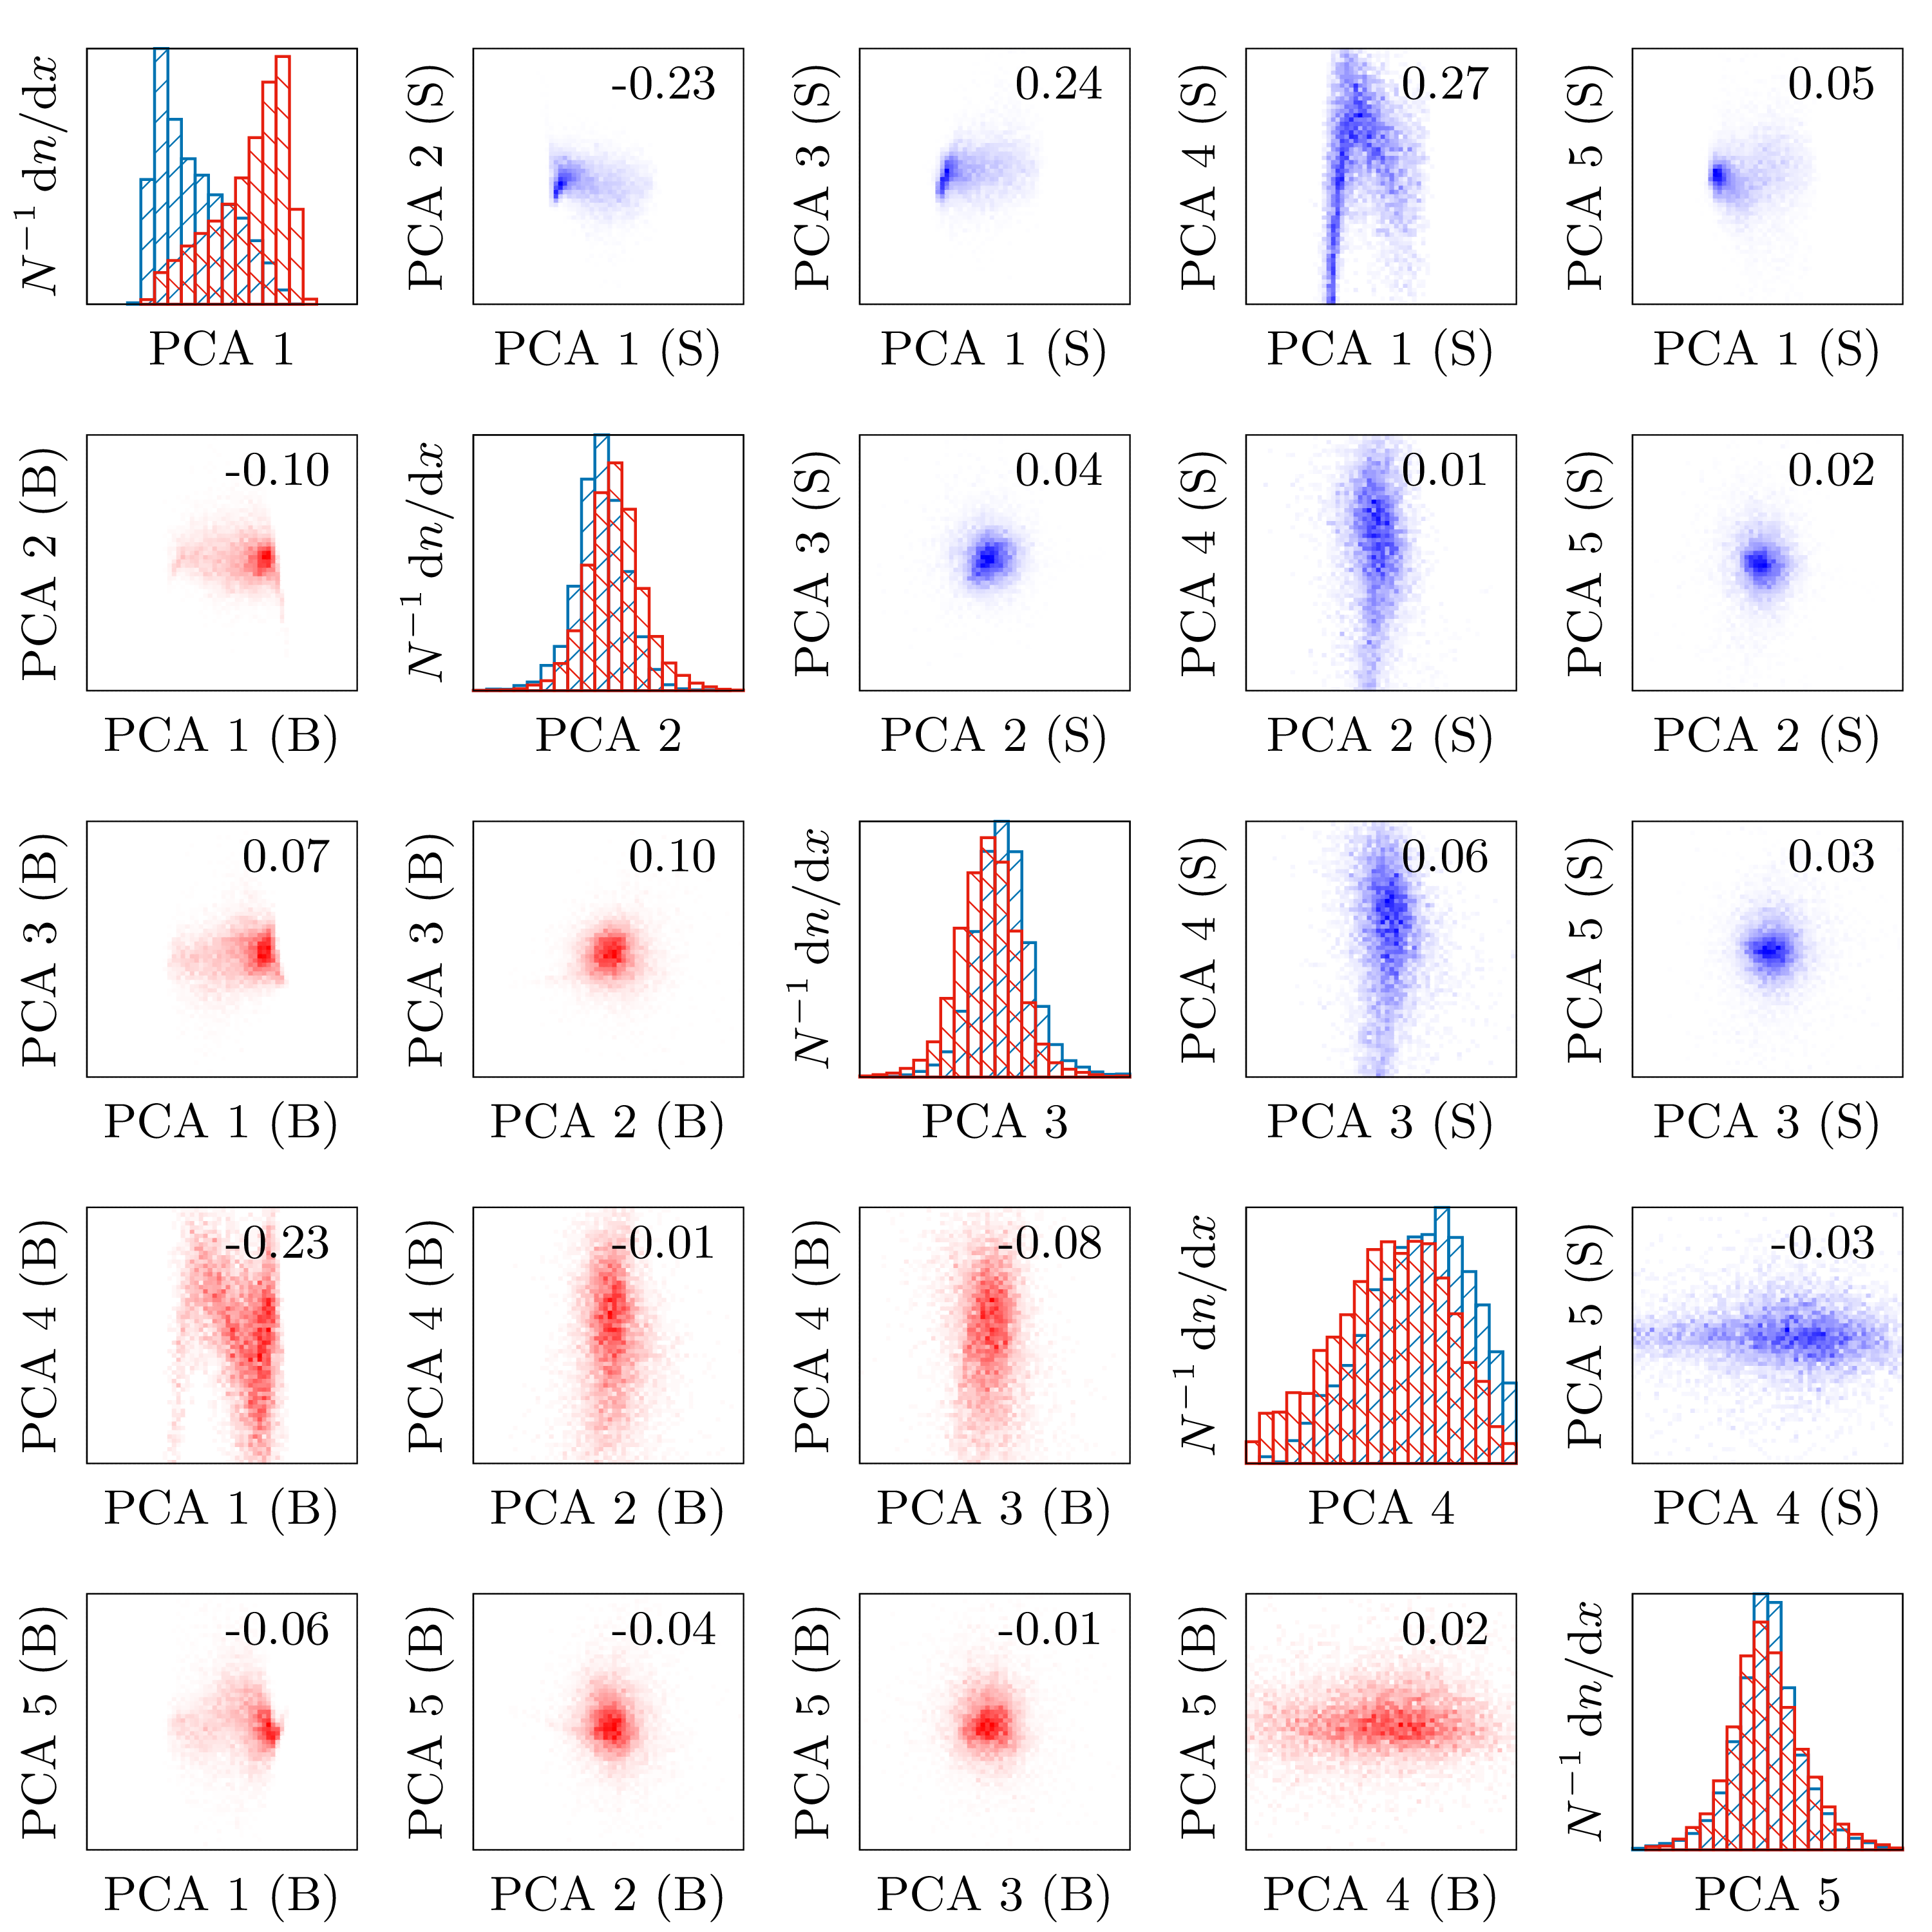
\includegraphics[height=.9\textheight]{mvaLz/stack_pcafeatures_DD}\\
            (track type \textbf{DD})
        \end{column}
    \end{columns}
\end{frame}

\begin{frame}{Fusion of high level classifiers}
    \begin{columns}
        \begin{column}{.5\textwidth}
            \centering
            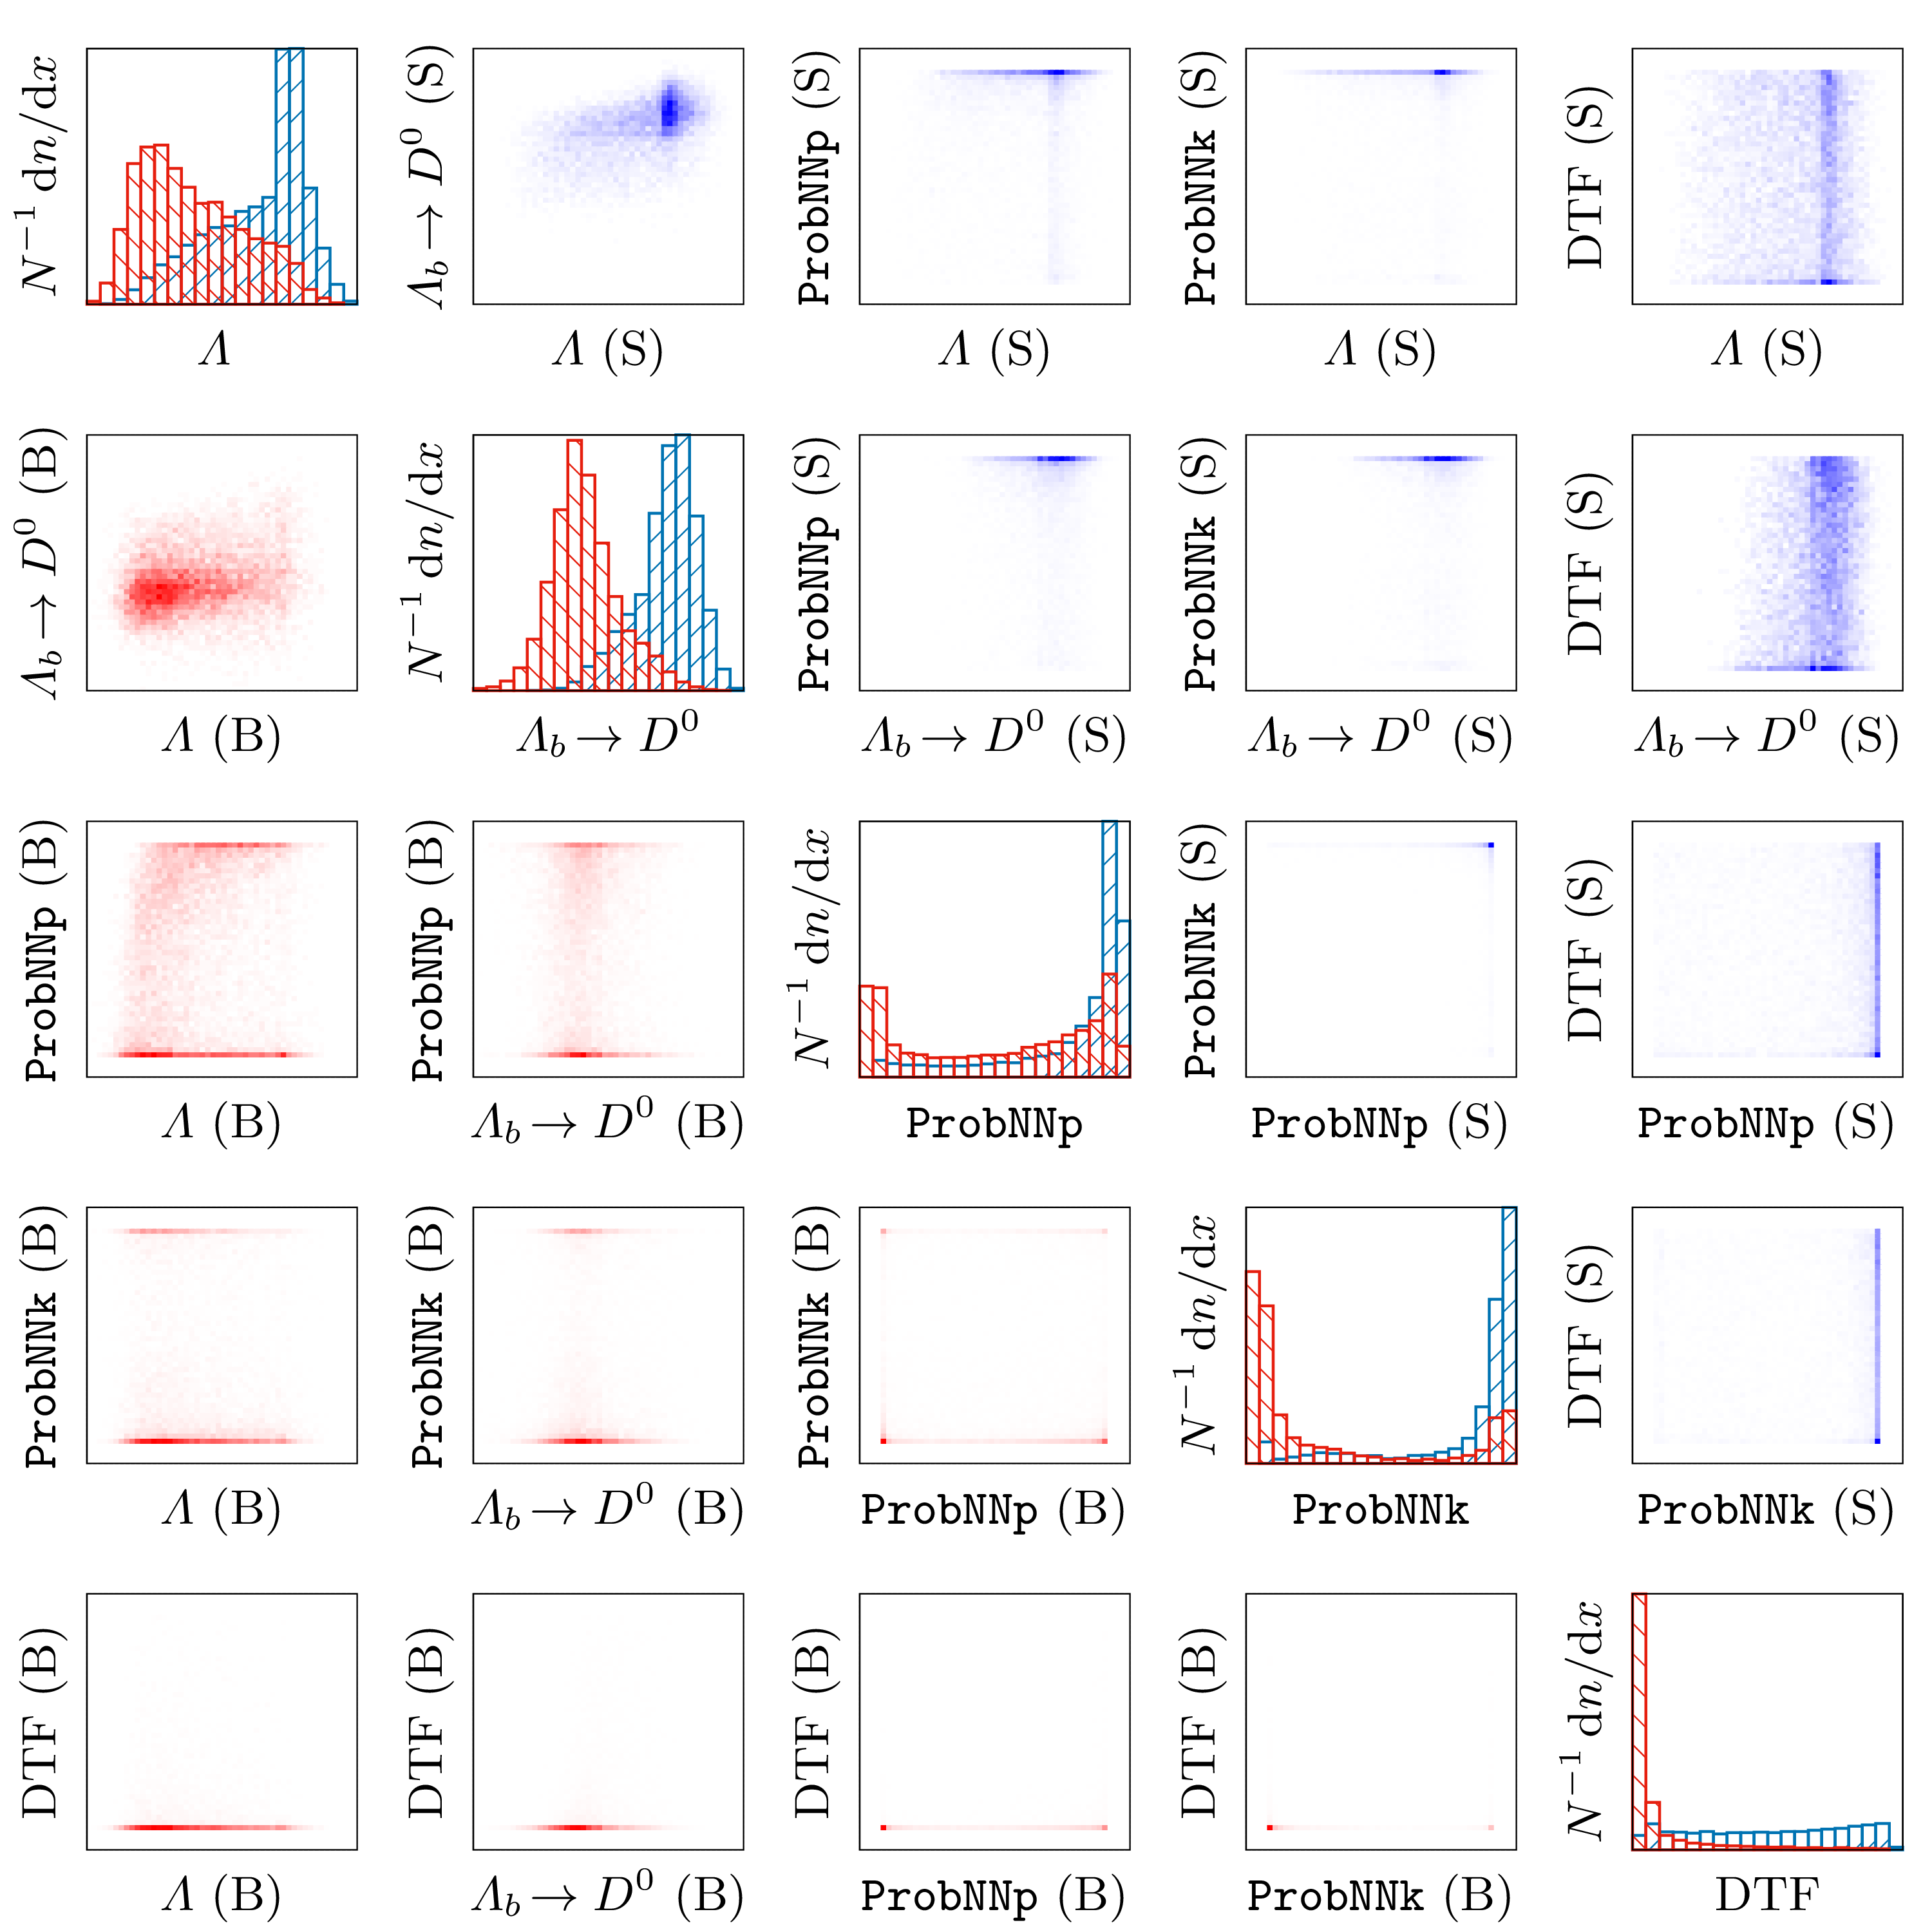
\includegraphics[height=.9\textheight]{mva/features_DD}\\
            (track type DD)
        \end{column}
        \begin{column}{.45\textwidth}
            \scalebox{1.2}{Fusion of high level classifiers}
            \begin{itemize}
                \item Optimize rectangular cut classifier (to avoid MC fidelity issues\ftntdagger)
                \item \ldots using classifier outputs as features
                \begin{enumerate}
                    \item \Lz classifier
                    \item \Lb-\Dz classifier
                    \item \texttt{ProbNNp}
                    \item \texttt{ProbNNk}
                    \item Decay tree fit
                \end{enumerate}
                \item (Compare rect.\ cut clf.\ eff.\ against decision tree\ftntdagger)
            \end{itemize}
        \end{column}
    \end{columns}
\end{frame}

\begin{frame}{Classifier fusion}
    \begin{columns}
        \begin{column}{.5\textwidth}
            \scalebox{1.2}{Optimize rect.\ cut clf.}
            \begin{itemize}
                \item Minimize FPR\ftnt{} at given TPR\ftnt\ftnt{}
                \item Numerically noisy: use simulated annealing for finding minimum 
                \item Set thresholds at TPR $\approx 50\,\%$ (LL) and TPR $\approx 30\,\%$ (DD)
                \item (Refine \textit{optimal} TPR with in a second, tight max.\ step only using $\Lz / \Lb$-$\Dz$ classifiers\ftntdagger)
            \end{itemize}
        \end{column}
        \begin{column}{.5\textwidth}
            \only<1>{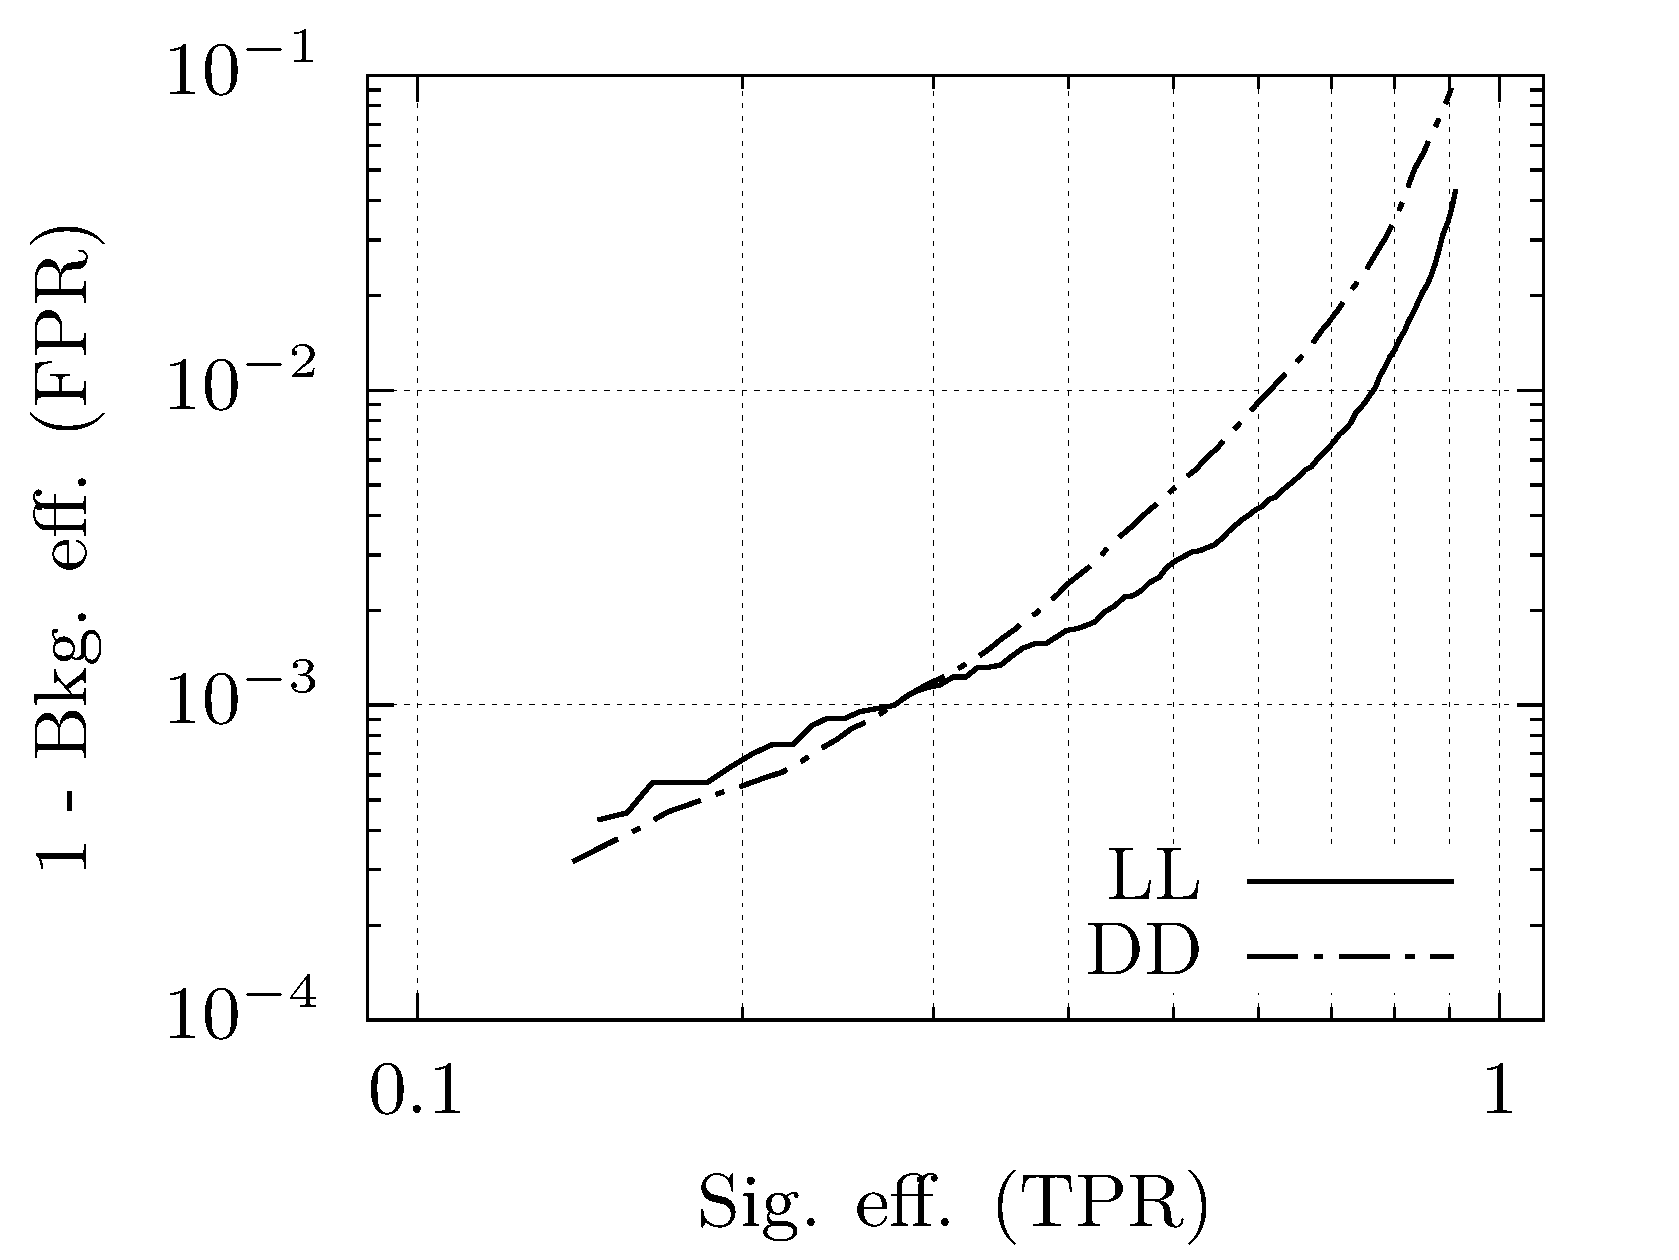
\includegraphics[scale=1.]{mva/roc}}%
            \only<2>{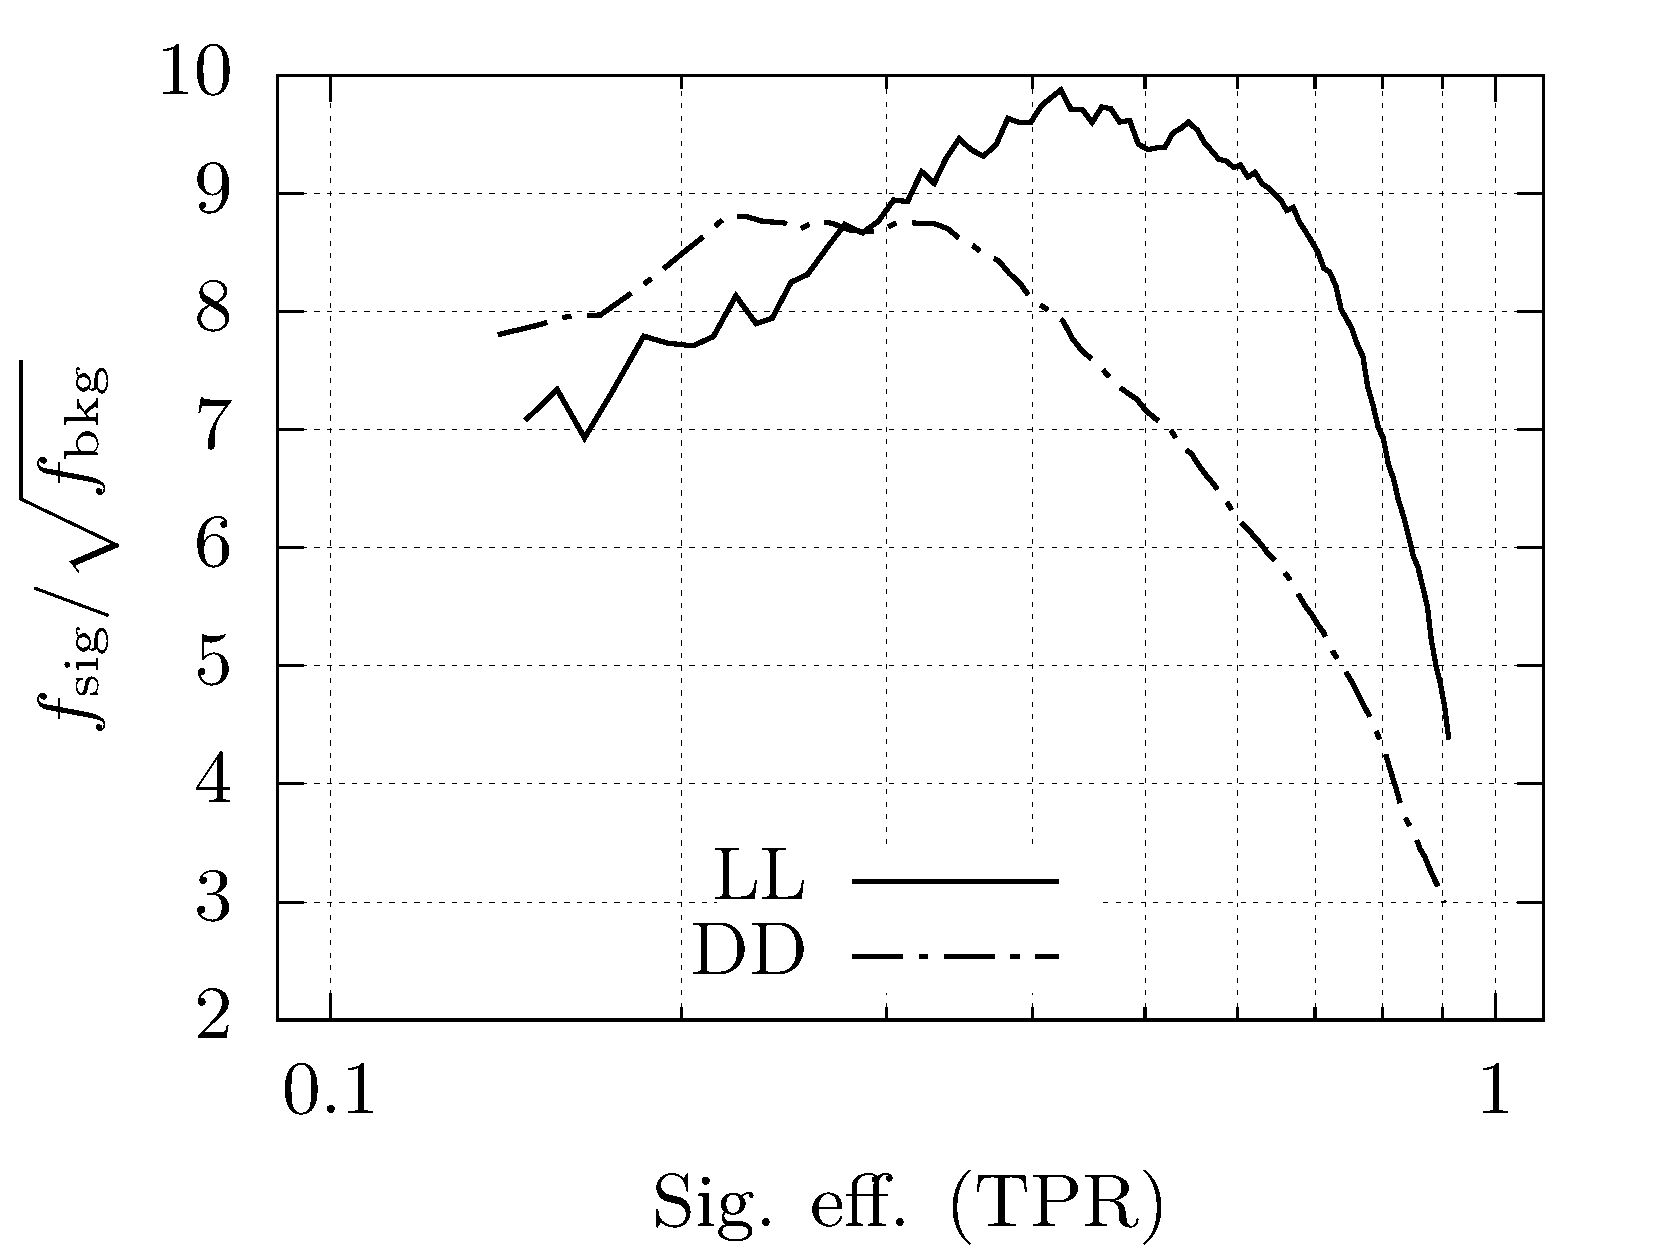
\includegraphics[scale=1.]{mva/significance}}%
        \end{column}
    \end{columns}

    \vspace{5mm}

    \footnotesize
    \phantom{\ftnt}\ftnt FPR: \underline{f}alse \underline{p}ositive \underline{r}ate, \ie{}, genuine bkg.\ predicted as sig.\\
    \ftnt\ftnt TPR: \underline{t}rue \underline{p}ositive \underline{r}ate, \ie{}, genuine sig.\ predicted as sig.
\end{frame}
